% ============================================================
% 5. RESULTS
% ============================================================
\section{Results}
\label{sec:results}

\subsection{Anomaly Detection Performance}
\label{sec:anomaly_results}

Table~\ref{tab:anomaly_results} presents the anomaly detection performance for the best configuration identified through our grid search: checkpoint \texttt{step\_100000}, $t_{\text{start}} = 150$, and guidance scale $w = 7.5$. This configuration achieves an image-level AUROC of 0.756 and AUPRC of 0.851, demonstrating meaningful discrimination between healthy and anomalous brain MRIs using only unsupervised training on healthy data.

\begin{table}[H]
\centering
\caption{Image-level anomaly detection performance (best configuration).}
\label{tab:anomaly_results}
\begin{tabular}{@{}lc@{}}
\toprule
\textbf{Metric} & \textbf{Value} \\
\midrule
AUROC        & 0.756 \\
AUPRC        & 0.851 \\
F1-Score     & 0.784 \\
Sensitivity  & 0.784 \\
Specificity  & 0.564 \\
Precision    & 0.783 \\
\bottomrule
\end{tabular}
\end{table}

At the pixel level, using ground truth polygon tumor masks, our model achieves a pixel-level AUROC of \textbf{0.894}, indicating strong localization capability. Figure~\ref{fig:roc_curve} shows the pixel-level ROC curve, and Figure~\ref{fig:qualitative} presents a qualitative example comparing the original MRI, ground truth tumor mask, and the generated anomaly heatmap.

\begin{figure}[H]
\centering
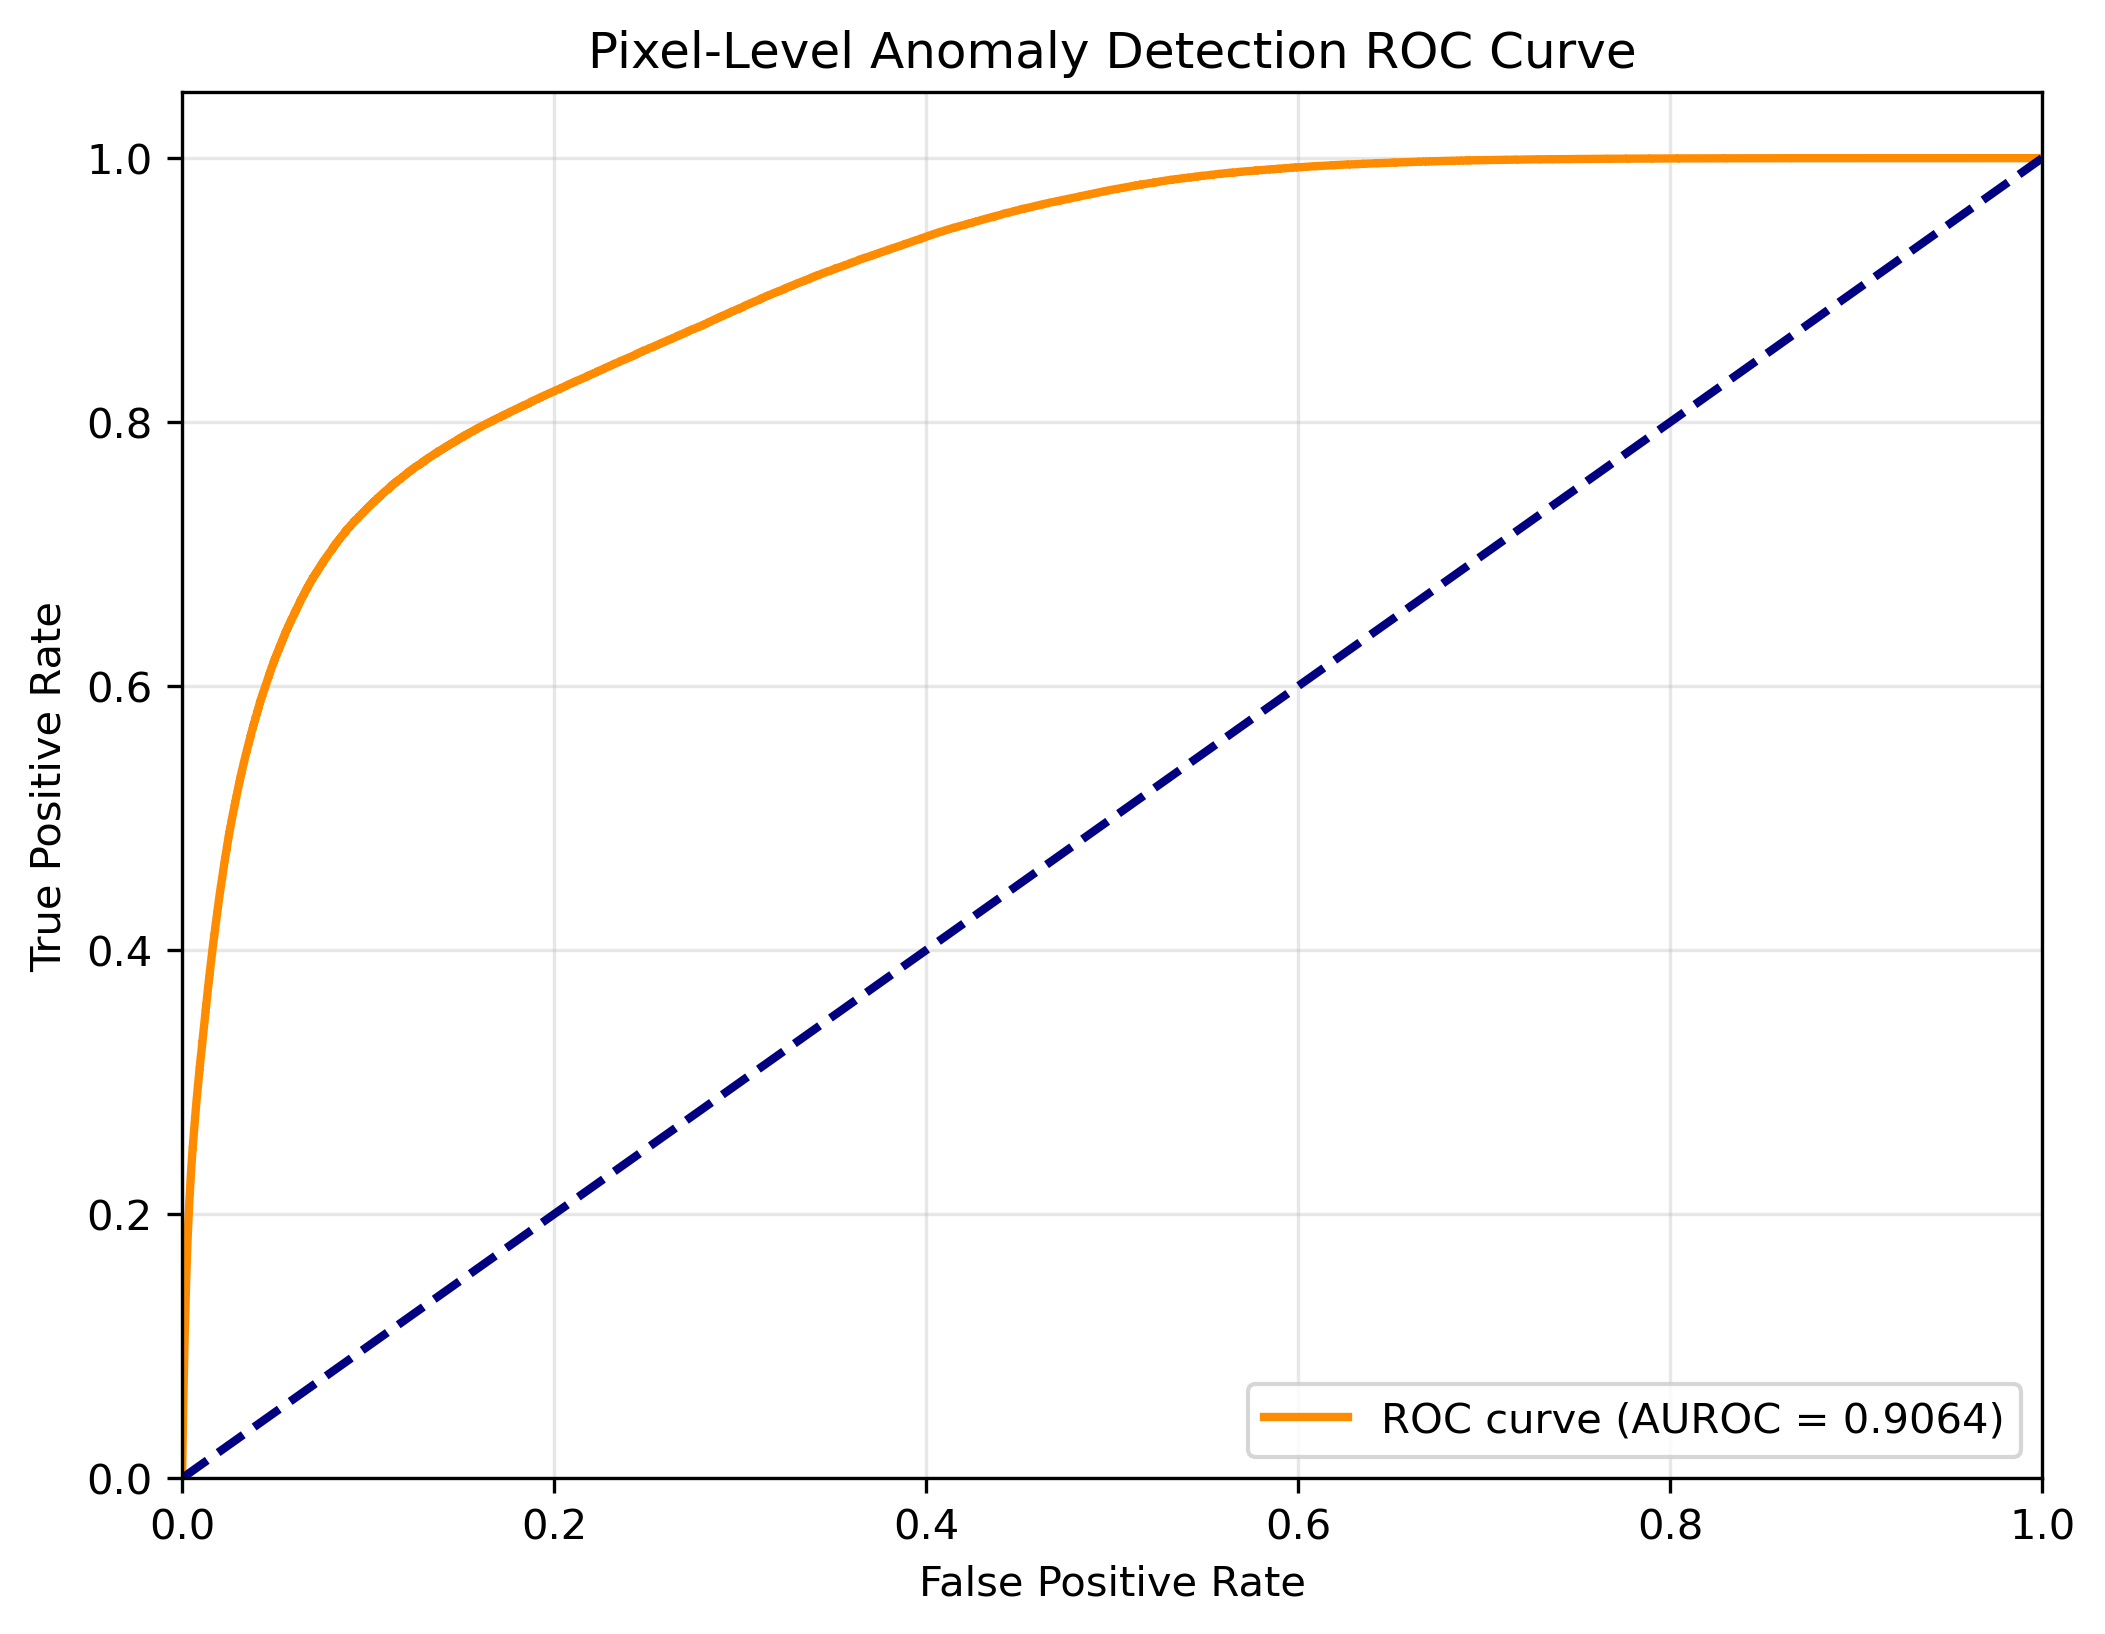
\includegraphics[width=0.65\textwidth]{../results/evaluation/roc_curve_pixel_level.png}
\caption{Pixel-level ROC curve for anomaly localization (AUROC = 0.894). The model demonstrates strong ability to discriminate tumor pixels from healthy tissue based on reconstruction error.}
\label{fig:roc_curve}
\end{figure}

\begin{figure}[H]
\centering
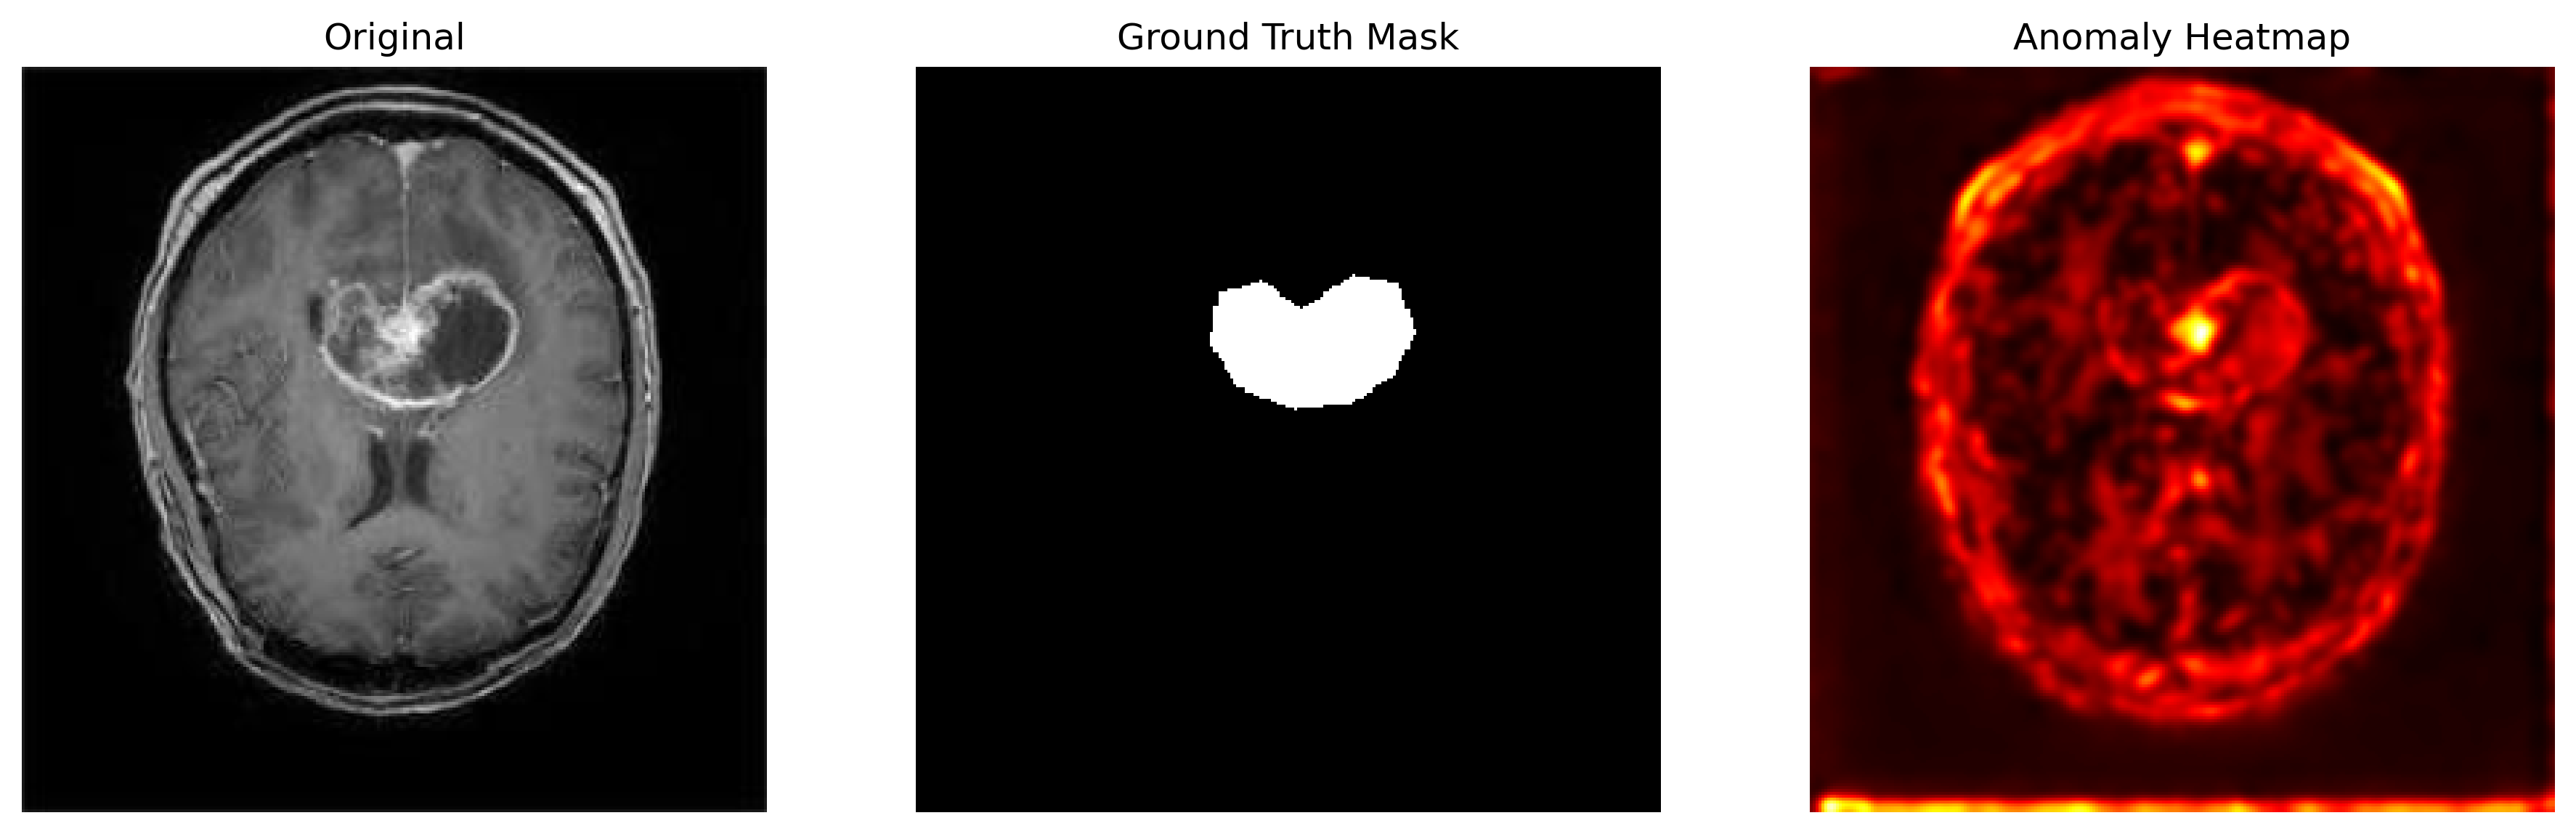
\includegraphics[width=0.95\textwidth]{../results/evaluation/qualitative_example.png}
\caption{Qualitative anomaly detection example. Left: original brain MRI with tumor. Center: ground truth tumor mask. Right: anomaly heatmap generated by our diffusion-based reconstruction pipeline. High-intensity regions in the heatmap correspond to areas where the healthy reconstruction deviates from the original, successfully localizing the tumor.}
\label{fig:qualitative}
\end{figure}

We also note that lowering the guidance scale to $w = 3.0$ (same checkpoint and $t_{\text{start}}$) yields a high-sensitivity configuration with sensitivity of \textbf{0.880} and F1 of 0.820, at the cost of reduced specificity (0.467). This trade-off is clinically relevant: a screening tool may prioritize sensitivity to avoid missing tumors, while a diagnostic tool may require balanced precision and recall.

\subsection{Hyperparameter Ablation Study}
\label{sec:grid_search}

We conducted an extensive grid search across 120 configurations: 10 training checkpoints (50K--140K steps, in 10K increments) $\times$ 4 noise injection levels ($t_{\text{start}} \in \{150, 200, 250, 300\}$) $\times$ 3 guidance scales ($w \in \{3.0, 5.0, 7.5\}$). Table~\ref{tab:top_configs} presents the top 5 configurations ranked by AUROC.

\begin{table}[H]
\centering
\caption{Top 5 hyperparameter configurations by image-level AUROC (grid search over 120 combinations).}
\label{tab:top_configs}
\begin{tabular}{@{}cccccccc@{}}
\toprule
\textbf{Checkpoint} & $\boldsymbol{t_{\textbf{start}}}$ & $\boldsymbol{w}$ & \textbf{AUROC} & \textbf{F1} & \textbf{Sens.} & \textbf{Spec.} \\
\midrule
step\_100K & 150 & 7.5 & \textbf{0.756} & 0.784 & 0.784 & 0.564 \\
step\_80K  & 200 & 7.5 & 0.755 & 0.754 & 0.711 & 0.649 \\
step\_100K & 150 & 3.0 & 0.755 & \textbf{0.820} & \textbf{0.880} & 0.467 \\
step\_140K & 150 & 3.0 & 0.755 & 0.785 & 0.784 & 0.573 \\
step\_100K & 150 & 5.0 & 0.755 & 0.742 & 0.689 & 0.662 \\
\bottomrule
\end{tabular}
\end{table}

\paragraph{Effect of Noise Injection Level ($t_{\text{start}}$).} The noise injection level emerges as the most critical hyperparameter. Table~\ref{tab:tstart_effect} shows performance at different $t_{\text{start}}$ values with the best checkpoint (step\_100K) and guidance scale ($w = 7.5$) held fixed. At $t_{\text{start}} = 150$, AUROC is maximized at 0.756. Higher values progressively degrade performance: at $t_{\text{start}} = 250$, AUROC drops to 0.739, and at $t_{\text{start}} = 400$, it falls to approximately 0.649. This confirms that excessive noising destroys healthy anatomical features along with pathology, while insufficient noising fails to remove the anomaly signal.

\begin{table}[H]
\centering
\caption{Effect of noise injection level $t_{\text{start}}$ on anomaly detection (step\_100K, $w = 7.5$).}
\label{tab:tstart_effect}
\begin{tabular}{@{}ccccc@{}}
\toprule
$\boldsymbol{t_{\textbf{start}}}$ & \textbf{AUROC} & \textbf{F1} & \textbf{Sensitivity} & \textbf{Specificity} \\
\midrule
150  & \textbf{0.756} & 0.784 & 0.784 & 0.564 \\
200  & 0.749 & 0.767 & 0.738 & 0.627 \\
250  & 0.739 & 0.793 & 0.811 & 0.529 \\
400  & 0.649 & 0.539 & 0.402 & 0.818 \\
\bottomrule
\end{tabular}
\end{table}

\paragraph{Effect of Guidance Scale ($w$).} The guidance scale exhibits a more nuanced effect: while AUROC remains relatively stable across guidance values (varying by less than 0.002), the guidance scale modulates the sensitivity--specificity trade-off. At $w = 3.0$, the model achieves the highest sensitivity (0.880) but lowest specificity (0.467); at $w = 7.5$, the balance shifts toward higher specificity (0.564) with moderate sensitivity (0.784). This behavior suggests that stronger guidance produces more conservative healthy reconstructions, reducing false positives at the cost of some false negatives.

\paragraph{Effect of Checkpoint Maturity.} The checkpoint at 100K training steps consistently produces the best AUROC across different hyperparameter combinations. Earlier checkpoints (50K--90K) show marginally lower AUROC, indicating incomplete convergence. Later checkpoints (110K--140K) show comparable but slightly reduced performance, suggesting mild overfitting to training data patterns.

\subsection{Synthetic Image Quality}
\label{sec:generation_results}

Table~\ref{tab:generation_metrics} presents the quantitative evaluation of 500 synthetic brain MRI images generated using checkpoint step\_100K with DDIM sampling (50 steps, $\eta = 0$, conditioned on healthy class).

\begin{table}[H]
\centering
\caption{Synthetic image generation quality metrics (500 generated images vs.\ real healthy test images).}
\label{tab:generation_metrics}
\begin{tabular}{@{}lc@{}}
\toprule
\textbf{Metric} & \textbf{Value} \\
\midrule
FID $\downarrow$                      & 144.43 \\
SSIM $\uparrow$                       & $0.129 \pm 0.085$ \\
LPIPS $\downarrow$                    & $0.534 \pm 0.033$ \\
Diversity (LPIPS) $\uparrow$          & $0.404 \pm 0.104$ \\
\bottomrule
\end{tabular}
\end{table}

The FID of 144.43 indicates moderate generation quality. While this is substantially higher than state-of-the-art natural image FID scores, it is important to contextualize this result: our model is trained on a relatively small dataset ($\sim$1,500 healthy images) of single-channel grayscale images at $256 \times 256$ resolution, and the FID metric (which uses ImageNet-pretrained Inception features) is less calibrated for medical grayscale imagery.

The intra-set diversity score (LPIPS = 0.404) confirms that the model generates varied samples rather than collapsing to a single mode, a common failure mode of GANs. The cross-distribution SSIM of 0.129 and LPIPS of 0.534 reflect the expected distributional distance between independently generated synthetic images and real images.

\subsection{Explainability Analysis}
\label{sec:explainability_results}

To enhance the interpretability of our model's predictions, we provide two complementary explainability mechanisms.

\paragraph{Self-Attention Maps.} Figure~\ref{fig:attention_maps} visualizes the self-attention weights extracted from the U-Net's attention layers at resolutions $16 \times 16$ and $8 \times 8$ during the denoising process. The attention maps reveal that the model learns to focus on anatomically meaningful structures---ventricular boundaries, cortical folds, and tissue interfaces---rather than attending uniformly across the spatial extent. This structured attention pattern provides evidence that the model has learned meaningful representations of brain anatomy.

\begin{figure}[H]
\centering
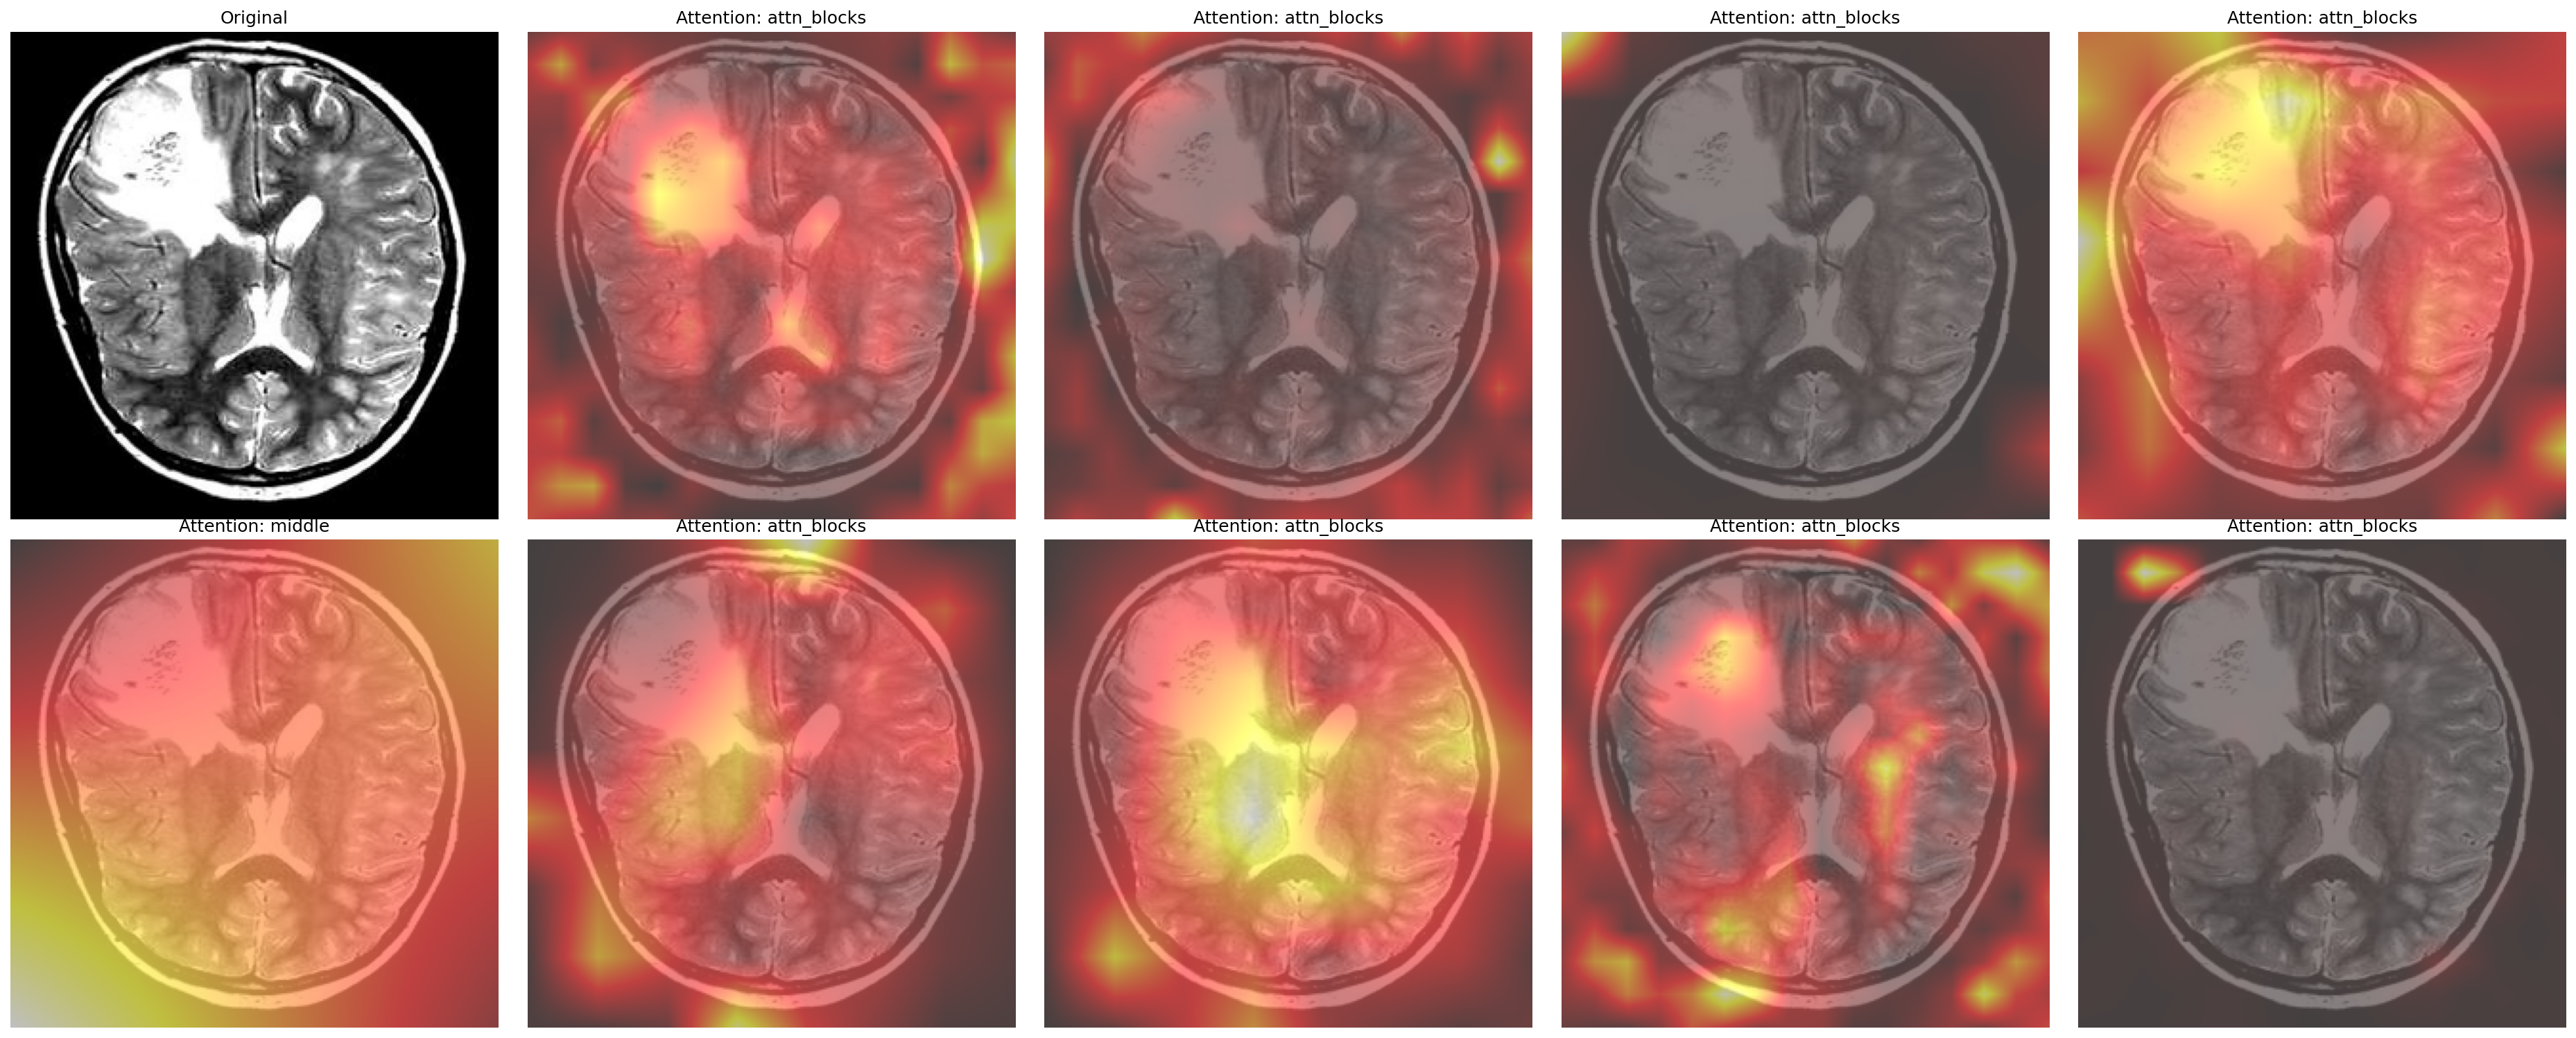
\includegraphics[width=0.95\textwidth]{../results/explainability/attention_maps.png}
\caption{Self-attention maps extracted from the U-Net during denoising. The model attends to anatomically relevant structures, demonstrating learned spatial awareness of brain morphology.}
\label{fig:attention_maps}
\end{figure}

\paragraph{Denoising Trajectory Comparison.} Figure~\ref{fig:denoising_trajectory} presents a side-by-side comparison of the denoising trajectory for a healthy and an anomalous brain MRI. The visualization shows intermediate decoded images at selected timesteps during the DDIM reverse process. For healthy inputs, the reconstruction converges smoothly to the original image. For anomalous inputs, the reconstruction progressively ``corrects'' the tumor region, replacing it with healthy-appearing tissue. This divergence between the original and reconstructed images in pathological regions is the mechanism underlying our anomaly detection approach.

\begin{figure}[H]
\centering
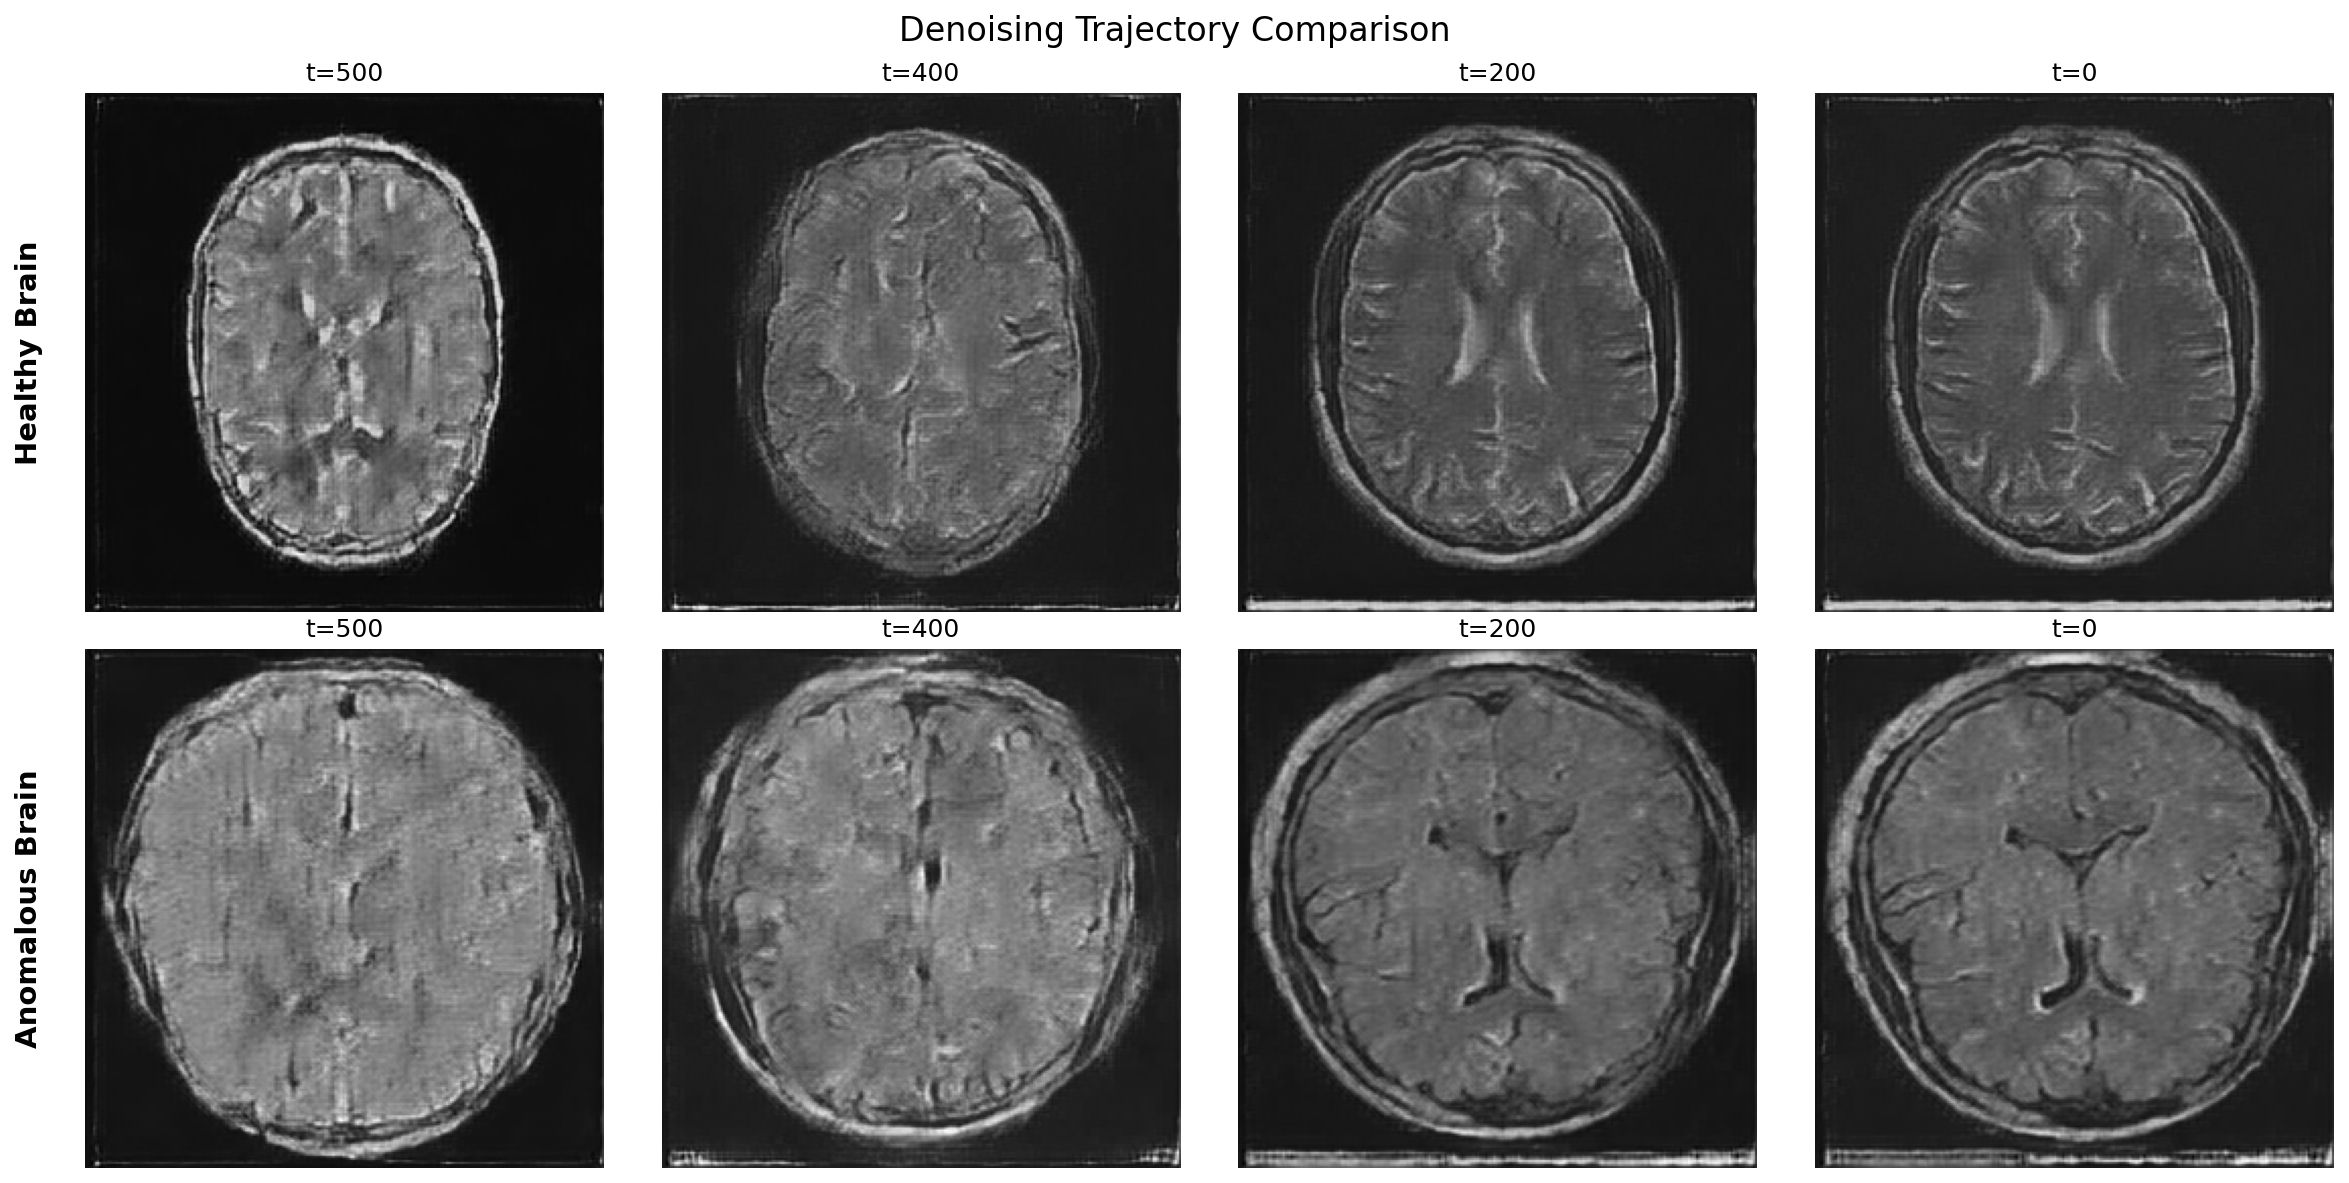
\includegraphics[width=0.95\textwidth]{../results/explainability/denoising_trajectory_comparison.png}
\caption{Denoising trajectory comparison between a healthy brain MRI (top) and a tumor-bearing MRI (bottom). The healthy-conditioned reconstruction progressively ``corrects'' the tumor region, generating the reconstruction error that drives anomaly detection.}
\label{fig:denoising_trajectory}
\end{figure}
